\documentclass{standalone}
\usepackage{tikz}
\usetikzlibrary{positioning, shapes, arrows.meta}

% Define variables
\newcommand{\verdist}{2cm}
\newcommand{\hordist}{4cm}

\begin{document}

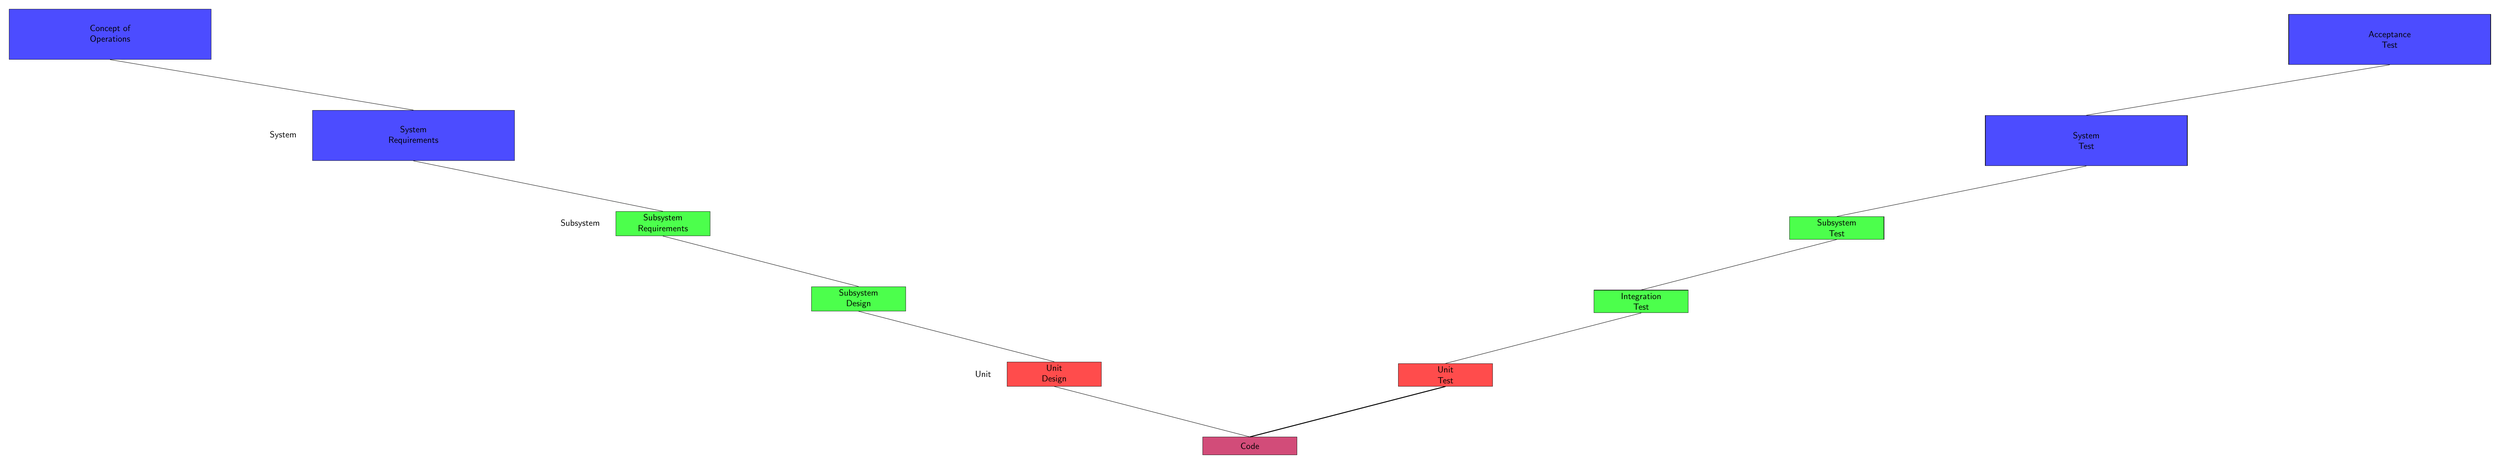
\begin{tikzpicture}[
  node distance=1.5cm and 2cm,
  every node/.style={font=\sffamily},
  process/.style={rectangle, draw, fill=blue!70, minimum width=8cm, minimum height=2cm, text width=3.5cm, text centered},
  process2/.style={rectangle, draw, fill=green!70, text width=3.5cm, text centered, minimum height=2em},
  process3/.style={rectangle, draw, fill=red!70, text width=3.5cm, text centered, minimum height=2em},
  process4/.style={rectangle, draw, fill=purple!70, text width=3.5cm, text centered, minimum height=2em},
  level/.style={anchor=south}
]

% Nodes
\node (concept) [process] {Concept of \\ Operations};
\node (sysreq) [process, below right=\verdist and \hordist of concept] {System \\ Requirements};
\node (subreq) [process2, below right=\verdist and \hordist of sysreq] {Subsystem \\ Requirements};
\node (subdesign) [process2, below right=\verdist and \hordist of subreq] {Subsystem \\ Design};
\node (unitdesign) [process3, below right=\verdist and \hordist of subdesign] {Unit \\ Design};
\node (code) [process4, below right=\verdist and \hordist of unitdesign] {Code};

\node (unittest) [process3, above right=\verdist and \hordist of code] {Unit \\ Test};
\node (integration) [process2, above right=\verdist and \hordist of unittest] {Integration \\ Test};
\node (subtest) [process2, above right=\verdist and \hordist of integration] {Subsystem \\ Test};
\node (systest) [process, above right=\verdist and \hordist of subtest] {System \\ Test};
\node (acceptance) [process, above right=\verdist and \hordist of systest] {Acceptance \\ Test};

% Connections
\draw[-] (concept.south) -- (sysreq.north);
\draw[-] (sysreq.south) -- (subreq.north);
\draw[-] (subreq.south) -- (subdesign.north);
\draw[-] (subdesign.south) -- (unitdesign.north);
\draw[-] (unitdesign.south) -- (code.north);

\draw[-,line width=1pt] (code.north) -- (unittest.south);
\draw[-] (unittest.north) -- (integration.south);
\draw[-] (systest.north) -- (acceptance.south);
\draw[-] (subtest.north) -- (systest.south);
\draw[-] (integration.north) -- (subtest.south);

% \draw[->] (code.east) -- ++(\verdist,0) |- (unittest.west);
% \draw[->] (unitdesign.east) -- ++(\verdist,0) |- (integration.west);
% \draw[->] (subdesign.east) -- ++(\verdist,0) |- (subtest.west);
% \draw[->] (subreq.east) -- ++(\verdist,0) |- (systest.west);
% \draw[->] (sysreq.east) -- ++(\verdist,0) |- (acceptance.west);

% Labels
\node[level, left=0.5cm of sysreq] {System};
\node[level, left=0.5cm of subreq] {Subsystem};
\node[level, left=0.5cm of unitdesign] {Unit};

\end{tikzpicture}

\end{document}
